\ifdefined\included
\else
\setcounter{chapter}{0}
\dominitoc
\faketableofcontents
\fi

\chapter{Human-Aware Navigation and Background}
\chaptermark{Human-Aware Navigation and Background}
\label{chap:1}
\minitoc

In this chapter, a formal definition of human-aware robot navigation is provided, followed by a description of the challenges involved. Then a brief explanation of how these challenges are currently addressed is provided. Further, we present the necessary background that is required to understand this thesis and then move on to the presentation of our approach. Before starting with HAN, we introduce general motion planning and robot navigation.

\section{Motion Planning and Robot Navigation}
In order to move a robot from one position to another, one should know the sequence of control commands that need to be sent to the robot. The intention behind any motion planning problem (manipulation or navigation) is to obtain a control sequence that a robot can execute to reach the goal pose from its initial (start) pose in a given environment while avoiding collisions. This is achieved by planning a collision-free path from the start to the goal first and then deriving feasible robot controls to trace the planned path as closely as possible. Hence the motion planning problem always requires the description of the environment (2D or 3D grids, maps etc.) and a goal position as inputs for path planning, while it requires the robot's kinematic description and dynamics for trajectory (or control) planning.  

Although both navigation and manipulation are motion planning problems and use similar algorithms, there are some basic differences. The navigation problem specifically deals with moving the entire robot from one place to another, whereas the manipulation problem deals with the motion of the end-effector and/or joints from the initial configuration to the goal configuration, while the base of the robot is assumed to be fixed. This thesis focuses only the navigation problem and specifically mobile robot navigation on ground using a 2D description of the world. Fig. \ref{fig:navigation} shows an example of such navigation planning avoiding the static obstacles in the environment.

\begin{figure}[!h]
    \centering
    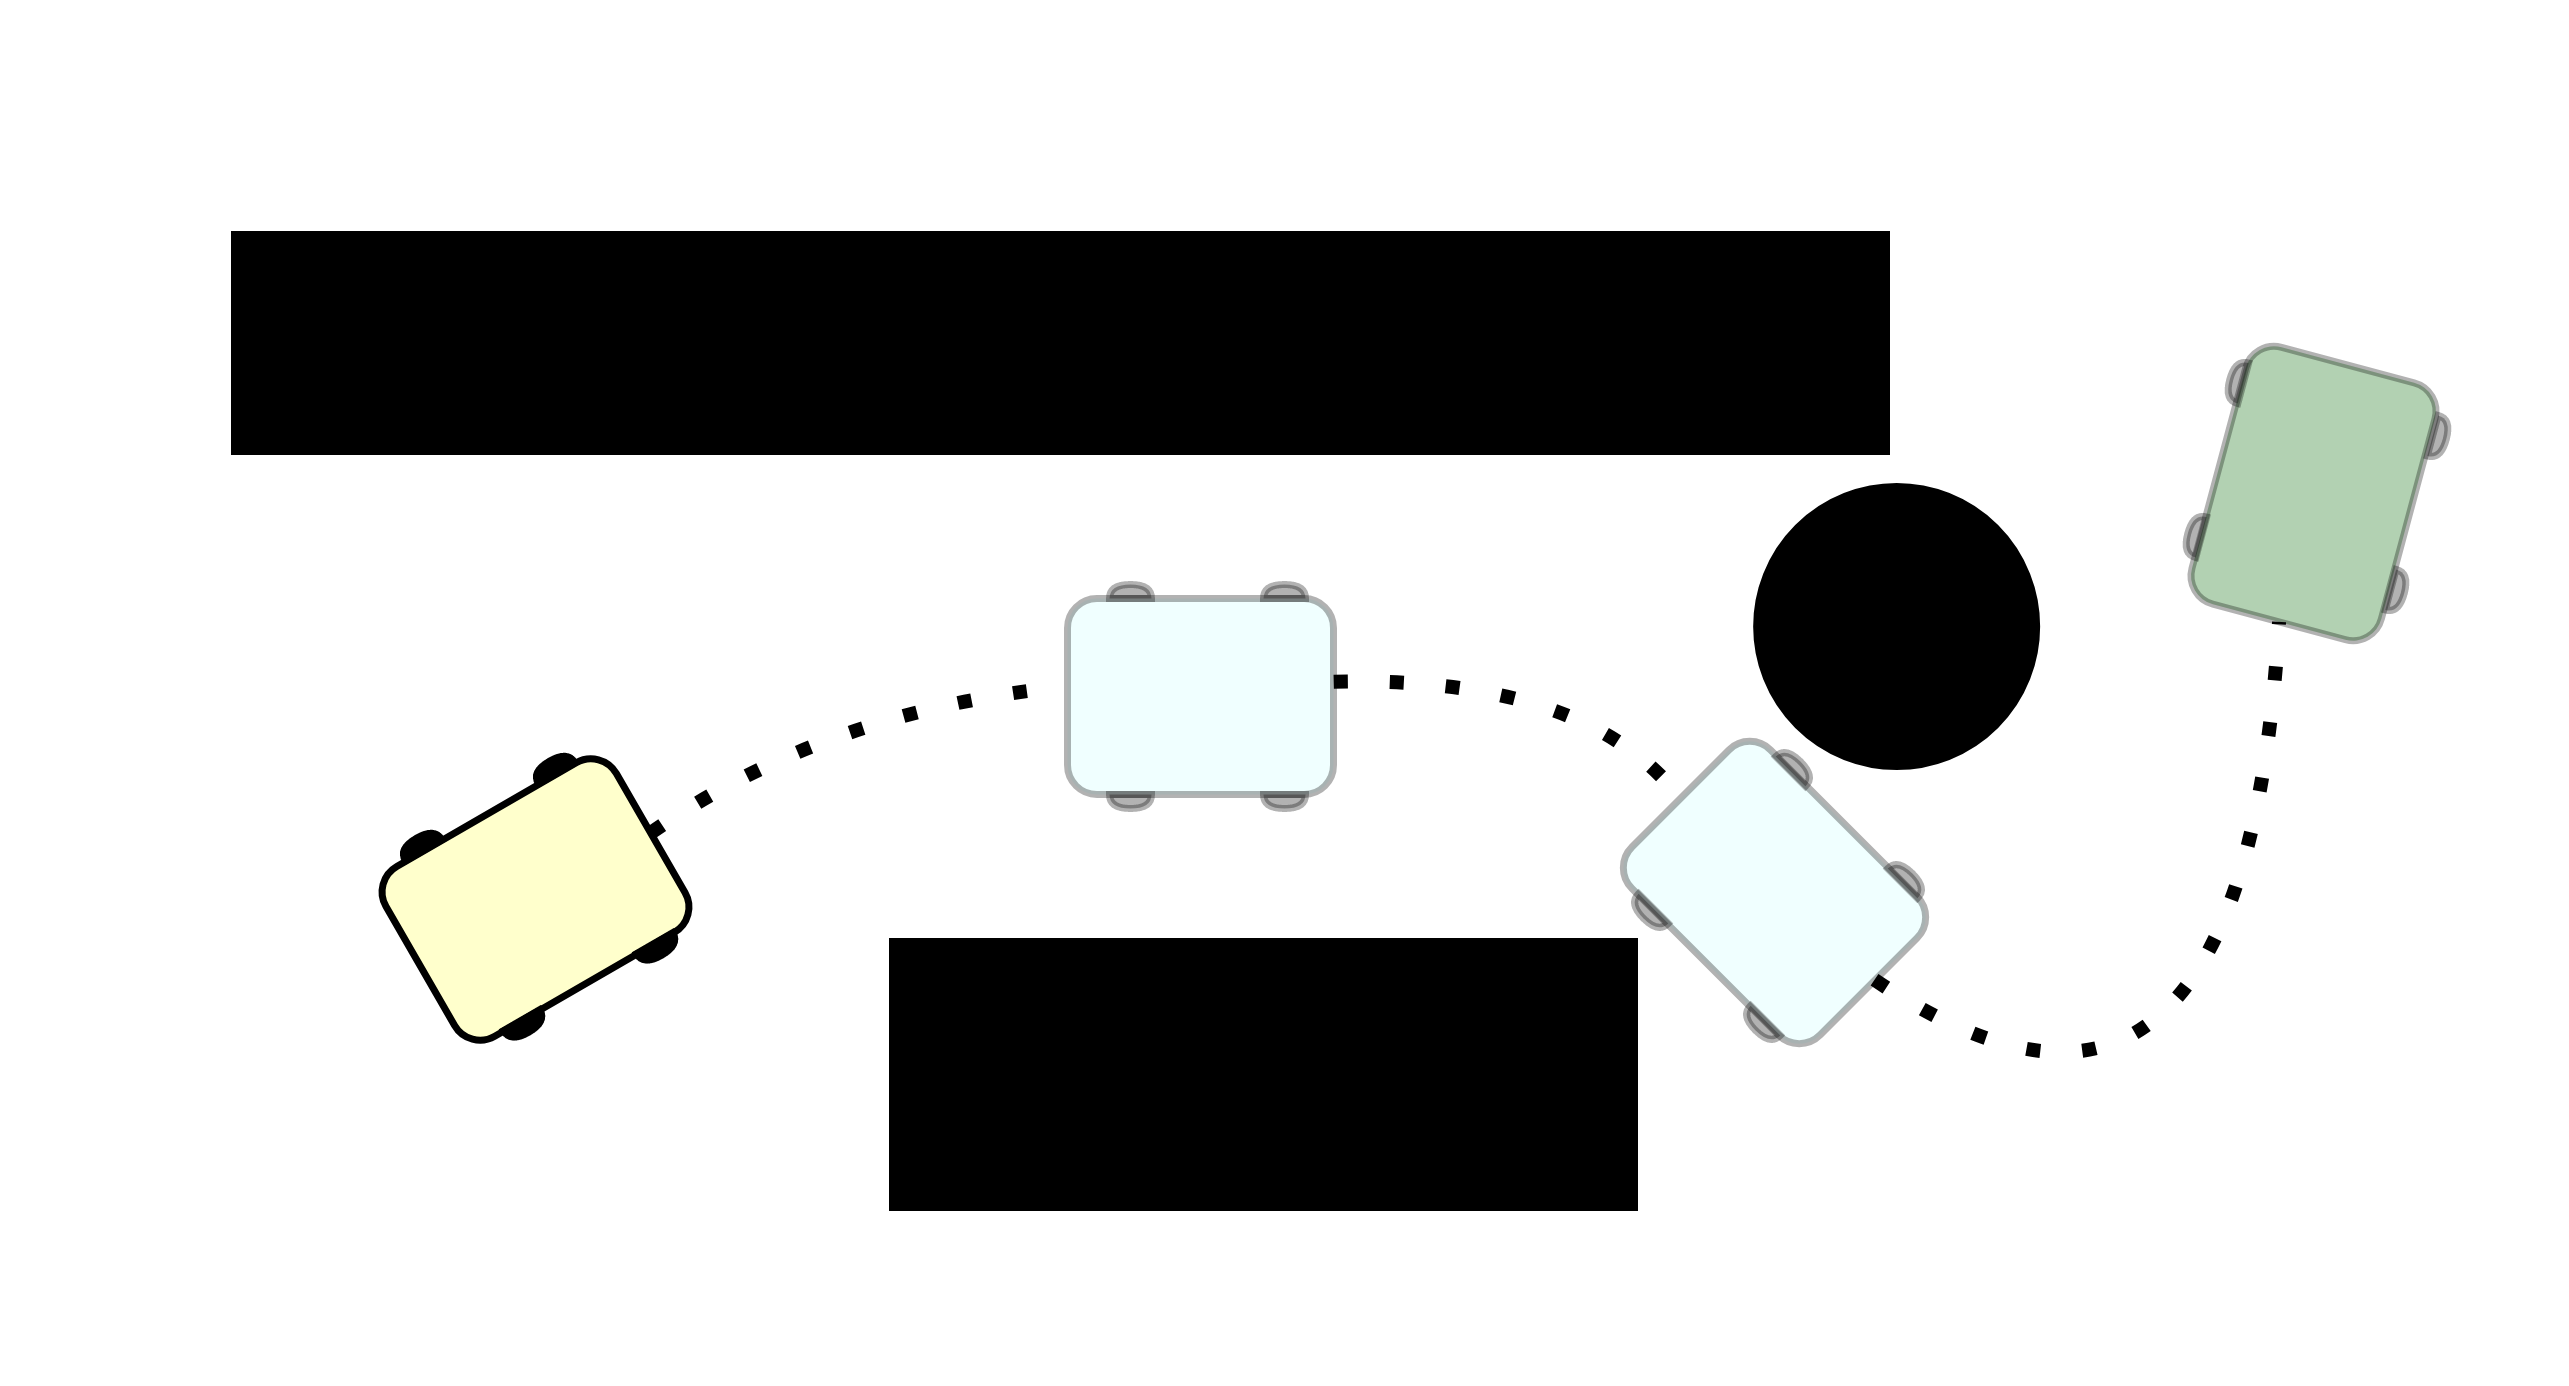
\includegraphics[width=0.9\columnwidth]{images/motion_planning_new.png}
    \caption{2D mobile robot Navigation from start (yellow) pose to goal (green) pose. The path planning problem has to plan the path and the intermediate poses (blue) that the robot needs to follow to reach the goal without colliding with the obstacles. The obstacles are marked in black. The trajectory planning then has to generate the control commands for the robot to follow this path.}
    \label{fig:navigation}
\end{figure}


As discussed previously, the robot navigation consists of path planning followed by trajectory planning to trace the planned path. The most commonly used approaches for path planning are either sampling-based \cite{lavalle2006sampling} or grid-based \cite{yap2002grid} graph searches with a sufficiently small step or grid size respectively. In a 2D setting with a static map, grid-based path finding algorithms like A* \cite{warren1993fast} are much faster compared to sampling-based approaches like RRT~\cite{kuffner2000rrt} or PRM~\cite{kavraki1996probabilistic}. Once a path is found, the next step is to find the feasible inputs for the robot's base controller to trace this path. Trajectory planning deals with this part while considering the kinodynamic limitations of the robot and other constraints. Hence it is often posed as an optimization problem with different optimality criteria like minimum time, minimum energy, or jerk \cite{gasparetto2015path}. One can employ any optimization technique like minimax~\cite{vathsal1977minimax}, genetic algorithms~\cite{tian2004effective}, multi-objective optimization~\cite{oleiwi2014multi}, unconstrained optimization~\cite{rosmann2013efficient}, or model predictive control~\cite{ardakani2015real} to solve this problem depending on the requirements. For robot navigation, trajectory planning has to be online and in real-time to handle the unexpected changes and dynamic obstacles in the environment. This thesis focuses on the online trajectory planning problem while relying on grid-based path planning (Dijkstra or A*) to generate the path.
%%%%%%%%%%%Paper%%%%%%%%%%%%%%%%%
% https://www.researchgate.net/profile/Paolo-Boscariol/publication/282955967_Path_Planning_and_Trajectory_Planning_Algorithms_A_General_Overview/links/59ad4b580f7e9bdd115c2afb/Path-Planning-and-Trajectory-Planning-Algorithms-A-General-Overview.pdf
%%%%%%%%%%%Paper%%%%%%%%%%%%%%%%%

\section{Human-Aware Navigation and the Challenges}

Human-Aware Robot Navigation (HAN) deals with the navigation planning of the robot in human workspaces. Therefore, it has to take into account several factors while planning. We believe that HAN needs to integrate human expectations, social norms and situation analysis into its planning while taking care of other static and dynamic obstacles. It should try to lessen the discomfort and make the robot motion more legible to the humans in the environment. However, there are several challenges associated with such planning, and some of them are presented here.

\subsection{The Challenges}
Being a multifaceted problem, HAN planning faces several challenges, and a single framework may not be able to provide a general solution to the problem. Some of the many challenges faced by HAN are given below. This may not be the complete list of challenges, but it comprises the majorly discussed issues in HAN. 
\begin{itemize}[leftmargin=*]
    % \item \textbf{\textit{Needs special obstacle modelling}}: Humans are not just dynamic obstacles. So, simple collision avoidance techniques are not sufficient. 
    % \item\textbf{ \textit{Hard to generalise}}: The robot’s motion should comply with certain social norms that change from place to place. Further, different humans and cultures react differently towards a robot.
    % \item \textbf{\textit{Requires decision making capabilities}}: The planning system needs to anticipate intentions and adjust the robot’s motion based on the context. 
    % \item \textbf{\textit{Needs communication}}: In order to negotiate a situation, some form of communication (gestures, signals etc.) needs to be included into the planning. We should also know when and what to communicate.
    % \item \textbf{\textit{No Standard metrics}}: As of today, there are no universally accepted metrics for human-aware navigation. More HRI studies must be conducted to determine these
    
    \item \textbf{\textit{Human Modelling}}: The most basic requirement for any HAN system is to have a model for a human navigating in the given environment. Treating humans as dynamic obstacles is not sufficient as a human have certain expectations and notions about other humans or agents in the environment. Therefore a special model is required for the human that is independent of place, culture, gender etc., and built over some common ground. 
    \item\textbf{\textit{Hard to Generalise}}: The robot navigation must comply with the social norms of the environment, and one of the major issues is that they change rapidly with human density, geometric context (corridor, door, open area etc.), place (office, warehouse, street etc.) and many other factors. Furthermore, each social norm requires a different way of modelling, and sometimes they could conflict with each other. Hence it is important to determine which social norms are relevant for the situation at hand. Lastly, people from different backgrounds react differently to the robot, and it adds more complexity to the planning.
    \item \textbf{\textit{Need for Decision-Making Capabilities}}: Without a proper situation assessment and handling, the robot could be contributing to the discomfort of humans rather than reducing it. Unless a HAN is designed to handle only a specific situation, it needs to evaluate the situation and take pertinent actions which require decision-making capabilities. The situation analysis also needs to anticipate possible actions and intentions of humans to avoid the occurrence of undesired situations and erratic behaviour of the robot. This requires good predictive models for human motion and intention detection.
    % As discussed above, the HAN system needs to anticipate the motion, intention and any sudden emergences of a human
    % The planning system needs to anticipate intentions and adjust the robot’s motion based on the context. 
    \item \textbf{\textit{Communication and Negotiation}}: The robot motion planned by a HAN system should not only respect the social norms but also needs to be legible. It requires the robot to show its navigation intention to the humans with or without explicit communication through the path or speed changes, gestures like waiting, turning to a side etc., signals and sometimes through voice or video. Explicit communication may also be needed to negotiate in intricate scenarios. The difficulty here is to know `when', `what' and `how' to communicate.
    % In order to negotiate a situation, some form of communication (gestures, signals etc.) needs to be included into the planning. We should also know when and what to communicate.
    \item \textbf{\textit{No Standard Metrics}}: As humans are social beings with different states of mind and backgrounds, it is difficult to come up with metrics that are applicable to every situation. Therefore, different researchers in HAN use different set of metrics for evaluation. Although there are some metrics that are widely used, they are not universally accepted and may be misleading in some contexts.
    
    % \item \textbf{\textit{Benchmarks and User Studies}}: 
    \textcolor{red}{Should I talk about benchmarks and user studies too?}
\end{itemize}

\subsection{Addressing the challenges}
As HAN has been a topic of research for quite some time, researchers have addressed the challenges in different ways. Human modelling was the first thing to be addressed. So, we start with it and then proceed to the robot planning.
\subsubsection{Human Model and Motion Prediction}
%%%%%%%%%%%Paper%%%%%%%%%%%%%%%%%
% Proxemics: https://link.springer.com/content/pdf/10.1007/s12369-014-0251-1.pdf
%%%%%%%%%%%%%%%%%%%%%%%%%%%%%%%%%
\begin{figure}[!h]
    \centering
    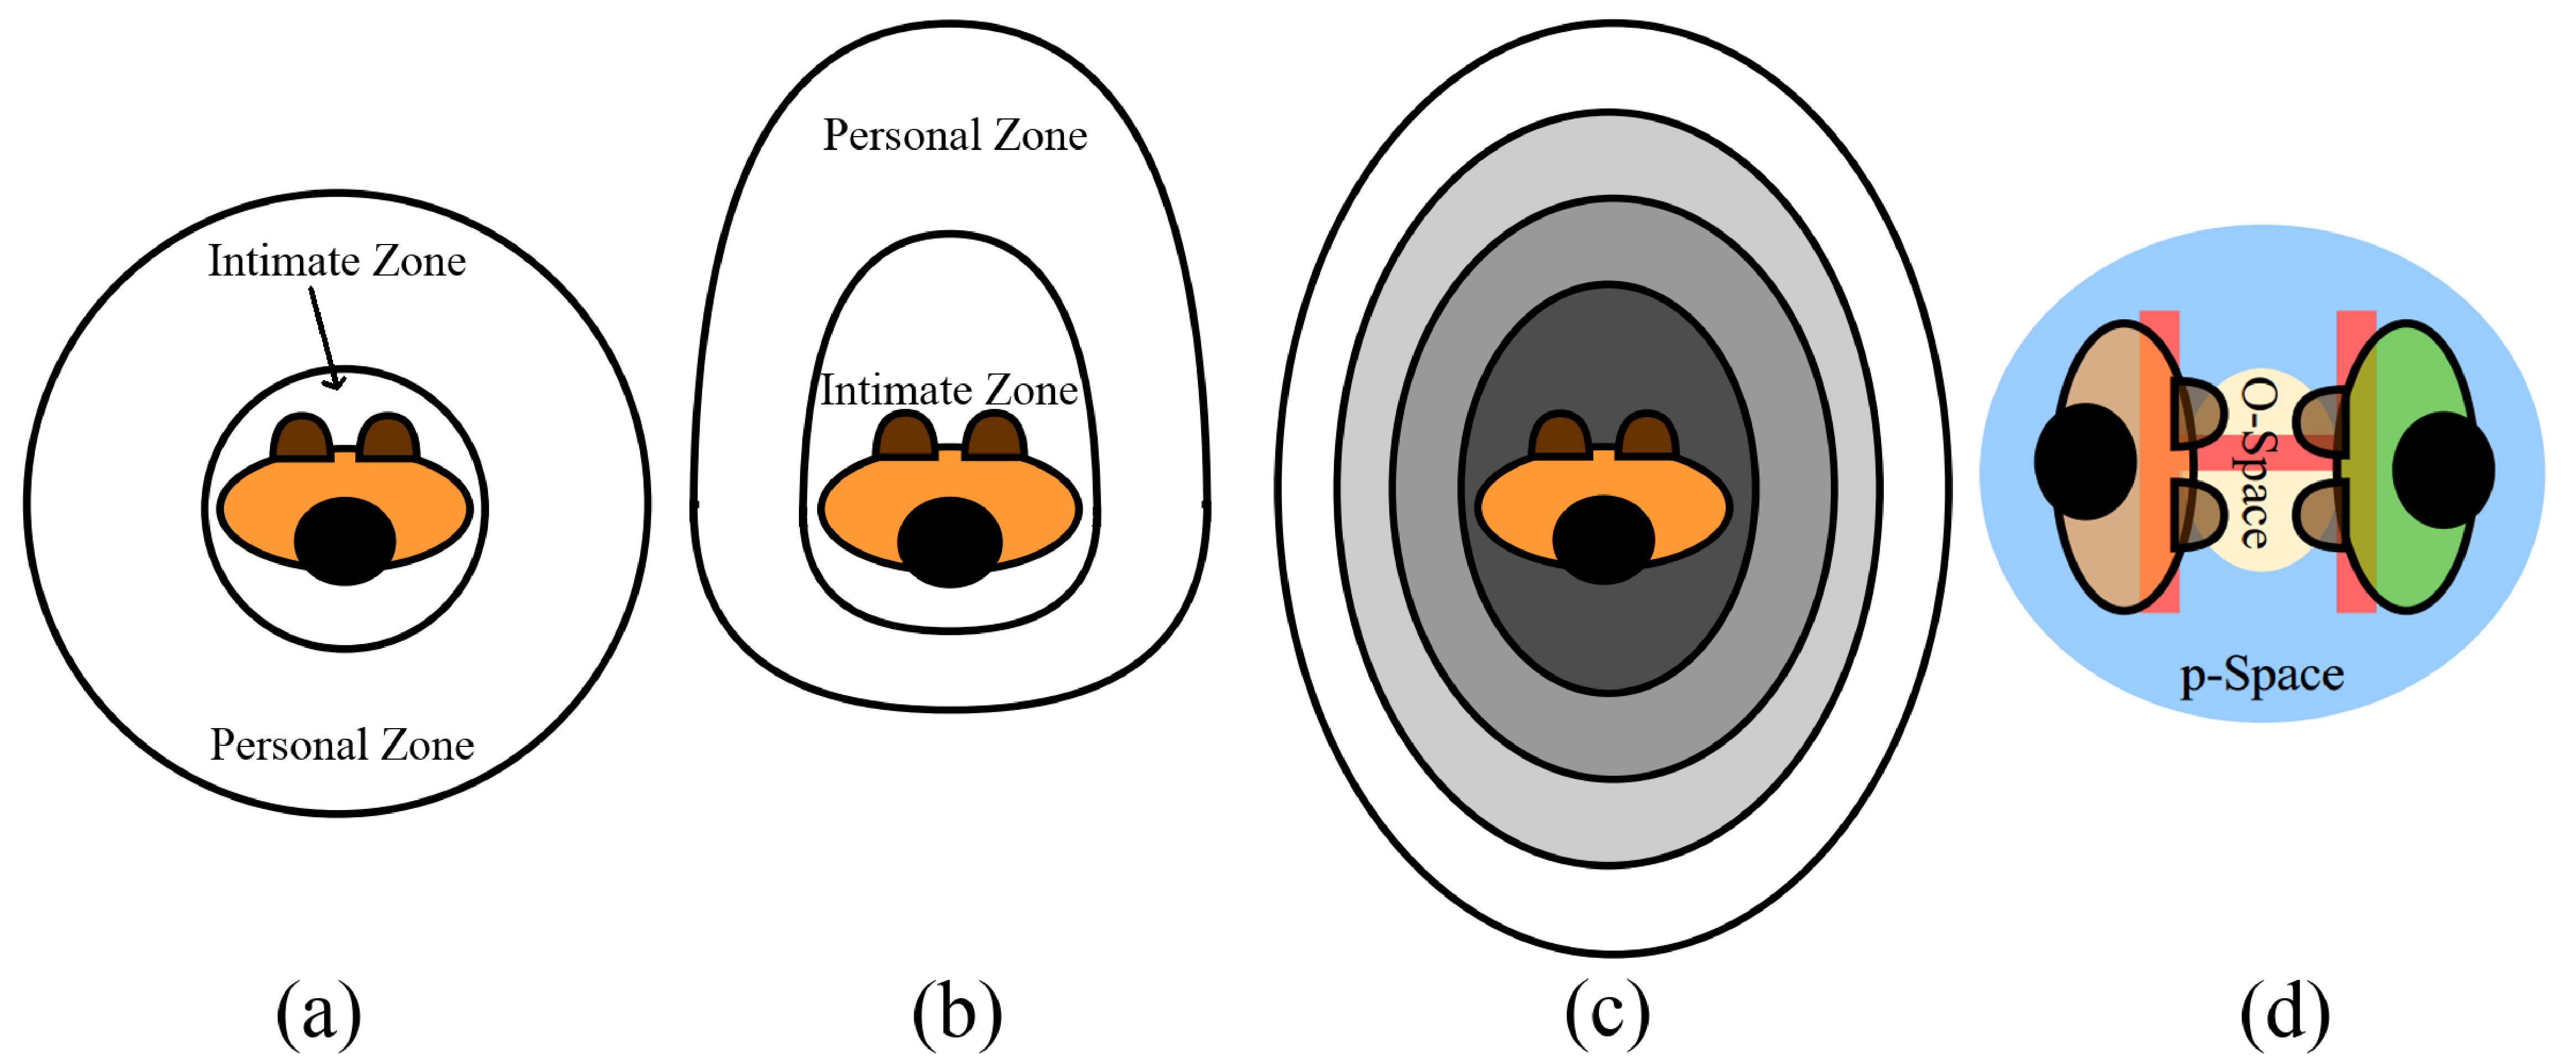
\includegraphics[width=0.95\columnwidth]{images/proxemics.eps}
    \caption{Zones and Spaces in Human and Group Modelling.}
    \label{fig:proxemics}
\end{figure}
For modelling humans, proxemics theory~\cite{mishra1983proxemics} provides some baselines that are common to most humans. Based on this, humans are designed as special obstacles with different zones around them. The very first modelling was done using concentric circles as shown in Fig. \ref{fig:proxemics} (a) with four different zones~\cite{rios2015proxemics}, namely, 1) the public zone ($> 3.6m$), 2) the social zone ($> 1.2m$), 3) the personal zone ($> 0.45m$) and 4) the intimate zone ($\leq 0.45m$). These measures are not very strict and vary with age, culture, background etc. The robot can interact and enter the public and social zones while it is prohibited from entering the personal and intimate zones. Later different shapes are proposed for these zones \cite{rios2015proxemics} and the most commonly used one these days is the \textit{Egg} shape shown in Fig. \ref{fig:proxemics} (b) that makes the robot maintain a larger distance towards frontal side compared to the sides or back. This is specifically true in the case of moving humans, and some works \cite{kostavelis2016human} adapt the shape based on the estimated human velocity. As Social Force Model \cite{helbing1995social} gained popularity in robotics, the human is assumed to have a repulsive potential field in the shape of an ellipse that is monotonically decreasing with a peak at the centre. Fig. \ref{fig:proxemics} (c) shows this shape and the decaying potential field. The direction of this field is the direction of motion of the human. As research progressed, different concepts like Information Processing Space~\cite{kitazawa2010pedestrian} and Object Affordance Spaces were introduced into the human model. For groups, the concepts of O-Spaces, p-Spaces and F-Formations \cite{rios2015proxemics} were introduced that allowed the robot to avoid, join or leave a group of humans appropriately. An example of O-Space and p-Space with \textit{Vis-a-Vis} (or H) F-formation is shown in Fig. \ref{fig:proxemics} (d). 

%%%%%%%%%%%%%%%Paper%%%%%%%%%%%
% https://link.springer.com/content/pdf/10.1007/978-3-642-04504-2.pdf
%%%%%%%%%%%%%%%%%%%%%%%%%%%%%%

It is necessary to predict the trajectory and motion of the human for the robot to act or react appropriately. As human detection and tracking is not the main focus of HAN, any off-the-shelf frameworks and systems can be used for this. After getting the necessary information about the humans' positions and velocities, a motion model is required to process these and predict the possible future trajectory. Thanks to the crowd navigation research, different methodologies like constant-velocity (or linear), ORCA~\cite{berg2011reciprocal}, Social Force \cite{helbing1995social}, Social-LSTM \cite{alahi2016social} etc., were used for the motion models and each one has its pros and cons. More methodologies and details are presented in the related work section. The trajectory prediction is done by forward simulating all the agents (humans and the robot) that are currently involved in HAN planning using their motion models (can be the same or different). Generally, the motion model has built-in collision avoidance strategies, and hence the predicted trajectories are collision-free. However, when simplistic models like Constant-Velocity are used, the trajectory prediction has to take care of collision avoidance as well.

%%%%%%%%%%%%%%Intention and Trajectory%%%%%%%%%%%%%
% Social Navigation Model based on Human Intention Analysis using Face Orientation
% You’ll Never Walk Alone: Modeling Social Behavior for Multi-target Tracking
% A Data-driven Framework for Proactive Intention-Aware Motion Planning of a Robot in a Human Environment
% A Review on Intention-aware and Interaction-aware Trajectory Prediction for Autonomous Vehicles
%%%%%%%%%%%%%%%%%%%%%%%%%%%%%%%%%%%%%%%
Human intention prediction is necessary to understand what humans might do in the future and take corrective actions. The meaning of intention may not be very clear as one can use it to refer to many things like whether the human is going to cross the sidewalk or not \cite{kohler2012early}, which direction the human will move or turn next~\cite{peddi2020data}, whether the human is willing to interact or not~\cite{ratsamee2013social} and many others. Although intention prediction will greatly benefit HAN, it is not very easy to predict and generalise. The recent advancements in machine learning and computer vision provided tools that can be used to predict intentions, and some works \cite{peddi2020data, ratsamee2013social} have already integrated it into HAN.

%%%%%%%%%%%%Paper : Goal Prediction %%%%%%%%%%%%
% https://dendorferpatrick.github.io/GoalGAN/
% https://upcommons.upc.edu/bitstream/handle/2117/26703/1462-Bayesian-Human-Motion-Intentionality-Prediction-in-Urban-Environments.pdf;jsessionid=5DC717935D7D9E75A0A0167020803AAD?sequence=1
%%%%%%%%%%%%%%%%%%%%%%%%%%%%%%%%%%%%%%%%%%%%%%%%%

\subsubsection{Robot Planning and Decision Making}
In the early stages, HAN planning was done by adding the proxemic zones around the humans and then planning a path that avoids intrusions into the personal and intimate zones. This mostly involved grid search (like A*) or potential field based path planning with simple controllers that tracked the path. In most of these settings, the humans and the groups are static while the robot navigates around them. 
With progress in dynamic obstacle avoidance, different strategies evolved for HAN, like continuous re-planning of the path with updated proxemic zones \cite{truong2014dynamic} and temporal planning \cite{kollmitz2015time}. However, scalability is an issue with such global planning strategies, which consider the entire 2D map and all possible states to re-plan or update the path. On the other hand, trajectory planning is mostly local and uses only a small portion of the map and states. This offered a better alternative for doing temporal or reactive planning in HAN, and consequently, a lot of works today focus on complex trajectory planning using simple path planning. As mentioned previously, trajectory planning problem always involves some kind of optimization (minimization or maximization) and naturally any kind of optimization techniques could be employed to solve this problem. The `\textit{human awareness}' is included in the robot's motion (or trajectory) through the constraints of optimization and sometimes they are referred to as `social or human-aware constraints'. Some commonly used optimization techniques in HAN include model predictive control \cite{rosmann2021online}, pareto-optimality \cite{forer2018socially}, graph optimization \cite{rosmann2013efficient} etc. However, there are other ways in which this problem is addressed and some popular approaches use Social Forces \cite{ferrer2013social}, Velocity Obstacles (ORCA and others) \cite{guzzi2013human}, Sampling based approaches like DWA \cite{fox1997dynamic} or RRT \cite{rios2011understanding} and Reinforcement Learning \cite{chen2017socially}. 

Trajectory planning in HAN should do more than simple collision avoidance with humans and obstacles. Since it is highly dependent on the context, it should best serve the task in the context rather than just avoiding discomfort. There it has to be tuned or planned to make the robot's motion legible and the interactions possible. One way to make robot's motion legible is through intention show using velocity or path modulation~\cite{kruse2014evaluating, lichtenthaler2013towards}, signals~\cite{may2015show} or visual projections~\cite{shrestha2018communicating}. All these have to be done while considering and following the social norms in the context. Some norms like `passing on right (or left)' could be employed using costmaps \cite{lu2013towards}, but some complex norms like waiting or advancing at a doorway to avoid blocking or giving way (moving to a side) for a human in a hurry require situation analysis and decision-making. Therefore many existing HAN systems employ state machines that switch between behaviours such as navigating in a crowd, approaching a human, following a human, standing in line etc., after analysing the situation. Some other recent works use POMDP \cite{qian2013decision} or deep learning  \cite{banisetty2020deep} based approaches to include these decision-making capabilities and behaviour switching into HAN.

% On the more practical side, several authors use state machines to switch between behaviors such as
% approaching a human, following the human, patrolling, searching, standing in line, and so on [1, 30, 35, 70,
% 81]. get references from the paper


In HRI, if the robot needs to communicate something or interact with the human, it needs to estimate `where' and `when' it should approach or meet the human and `how' it should plan its trajectory to be legible to all the humans in the environment (or context). Such things are usually addressed using Inverse Reinforcement Learning \cite{ramirez_robots_2016} or potential fields \cite{hansen2009adaptive}. Unlike in-place interactions that take place in some HRI tasks, HAN has to communicate (voice or gestures) while it is navigating to negotiate or prevent the occurrence of freezing robot problem. This is usually done by maintaining a knowledge-base and a model \cite{dugas2020ian} that decides `what' and `when' to communicate. This again emphasises the need for decision-making in HAN.


% So human-awareness is represented in localplanners mostly by interleaving prediction of human motion
% and planning or robot motion to identify potentials for joint efforts in collision avoidance.

\section{Background}
In this section, we provide details on some of the tools and mathematical modelling that is necessary to understand our approach to HAN planning.  

\subsection{ROS Navigation Stack}
Robot Operating System (ROS) \cite{quigley2009ros} provides an environment to develop different tools for robotic platforms. It has several built-in packages and software bundles that make this development easier. Being an open-source platform, there are several custom packages and large community support to discuss and resolve issues. ROS readily supports motion planning and has official packages for navigation as well as manipulation. As the HAN system presented in this thesis is developed using the ROS Navigation Stack\footnote{\url{http://wiki.ros.org/navigation}}, we briefly present its features. The main package of this stack is \textit{\textbf{move\_base}} that provides the plugins to include new planners.

\textbf{Inputs}: Apart from the 2D navigation goal (position and orientation), the navigation stack takes as input the odometry information, the sensory data like laser or point cloud to obtain the real-time obstacle information and the static map data for planning the path. It also requires the necessary transformation to connect the `\textit{map}' and the `\textit{base\_link}' of the robot, which usually is published by the localisation module.

\textbf{Architecture}: The navigation stack has a `\textit{global planner}' that takes care of the path planning and a `\textit{local planner}' that deals with the trajectory planning. Both these planners are built as plugins and provide an easy way to use your own custom planners besides the existing ones. As it is built over ROS, the parameters and the planners can be updated easily using the `\textit{yaml}' configuration files. 

\textbf{Output}: It outputs the command velocity for the robot's base controller.

\subsection{Timed Elastic Band for Trajectory Planning}
Timed-Elastic Band (TEB) for trajectory planning is proposed in \cite{rosmann2013efficient} and is available as one of the local planners\footnote{\url{http://wiki.ros.org/teb_local_planner}} in ROS. This approach uses hypergraph representation to build the timed-elastic band and then optimizes the graph to get the optimal command velocity.
\subsubsection{TEB Formulation}
The robot's trajectory in 2D navigation can be represented as a sequence of $n$ poses, $p_i = (x_i, y_i, \theta_i) \in \mathbb{R}^2 \times S^1$  and with a set of $n-1$ time intervals, $\delta t_i \in \mathbb{R}^+$ between two consecutive poses. Classically, in an elastic band \cite{quinlan1993elastic} approach, only the poses were considered along with the kinematic model of the robot, and therefore, the obtained trajectory may not satisfy the dynamic constraints of the robot. On the other hand, TEB considers both poses and time intervals and hence, the resultant trajectory is both kinematically and dynamically feasible. Let the sequence of poses, $\{p_i\}$, and the time intervals $\{\delta t_i\}$ be represented by:
\begin{equation*}
    \begin{aligned}
      P & = \{p_i\}_{i=0...n} \quad n \in \mathbb{N} \\
      \tau & = \{\delta t_i\}_{i=0..n-1} 
    \end{aligned}
\end{equation*}

Using these sequences, $P$ and $\tau$, TEB is defined as a tuple:
\begin{equation}
    B := (P,\tau)
\end{equation}

TEB is then optimized using a weighted multi-objective optimization to obtain the optimal poses and time intervals in real-time:
\begin{equation}
    f(B) = \sum_k \alpha_kf_k(B)
\end{equation}
\begin{equation}
    B^* = \argmin_B f(B)
\end{equation}
where $f(B)$ is the objective function, $B^*$ denotes the optimized TEB. The objective function $f(B)$ is a weighted (by $\alpha_i$) sum of different components $f_k(B)$ that represent different kinodynamic constraints. The constraints are formulated as objectives in terms of a piecewise continuous, differential cost function that penalises the violation of a constraint \cite{rosmann2013efficient}.

%%%%%%%%Can be a part of g2o intro
%  Most of these constraints ($f_i(B)$) are local as they depend only on a few number of consecutive configurations rather than the entire band, B and this property of TEB results in a sparse system matrix.

\subsubsection{Hypergraphs and TEB Hypergraph}
Hypergraph is a generalised graph with hyperedges \cite{bretto2013hypergraph} that can connect any number of vertices (or nodes) unlike a normal graph where an edge connects only two vertices.
% \begin{figure}[!h]
%     \centering
%     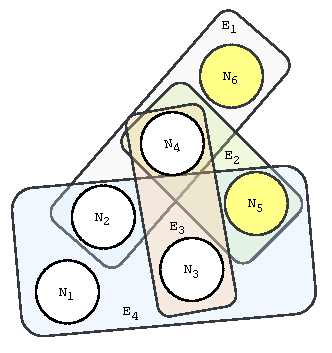
\includegraphics[width=0.4\columnwidth]{images/hypergraph.png}
%     \caption{An example hypergraph with 4 hyperedges and 6 nodes}
%     \label{fig:hypergraph}
% \end{figure}\\
\begin{figure}[!h]
    \centering
    \begin{subfigure}[t]{0.45\columnwidth}
        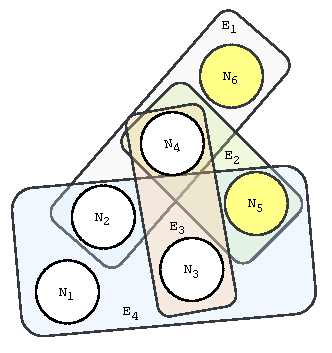
\includegraphics[width=0.9\textwidth]{images/hypergraph.png}
    \caption{A general hypergraph}
    \end{subfigure}
     \begin{subfigure}[t]{0.45\columnwidth}
        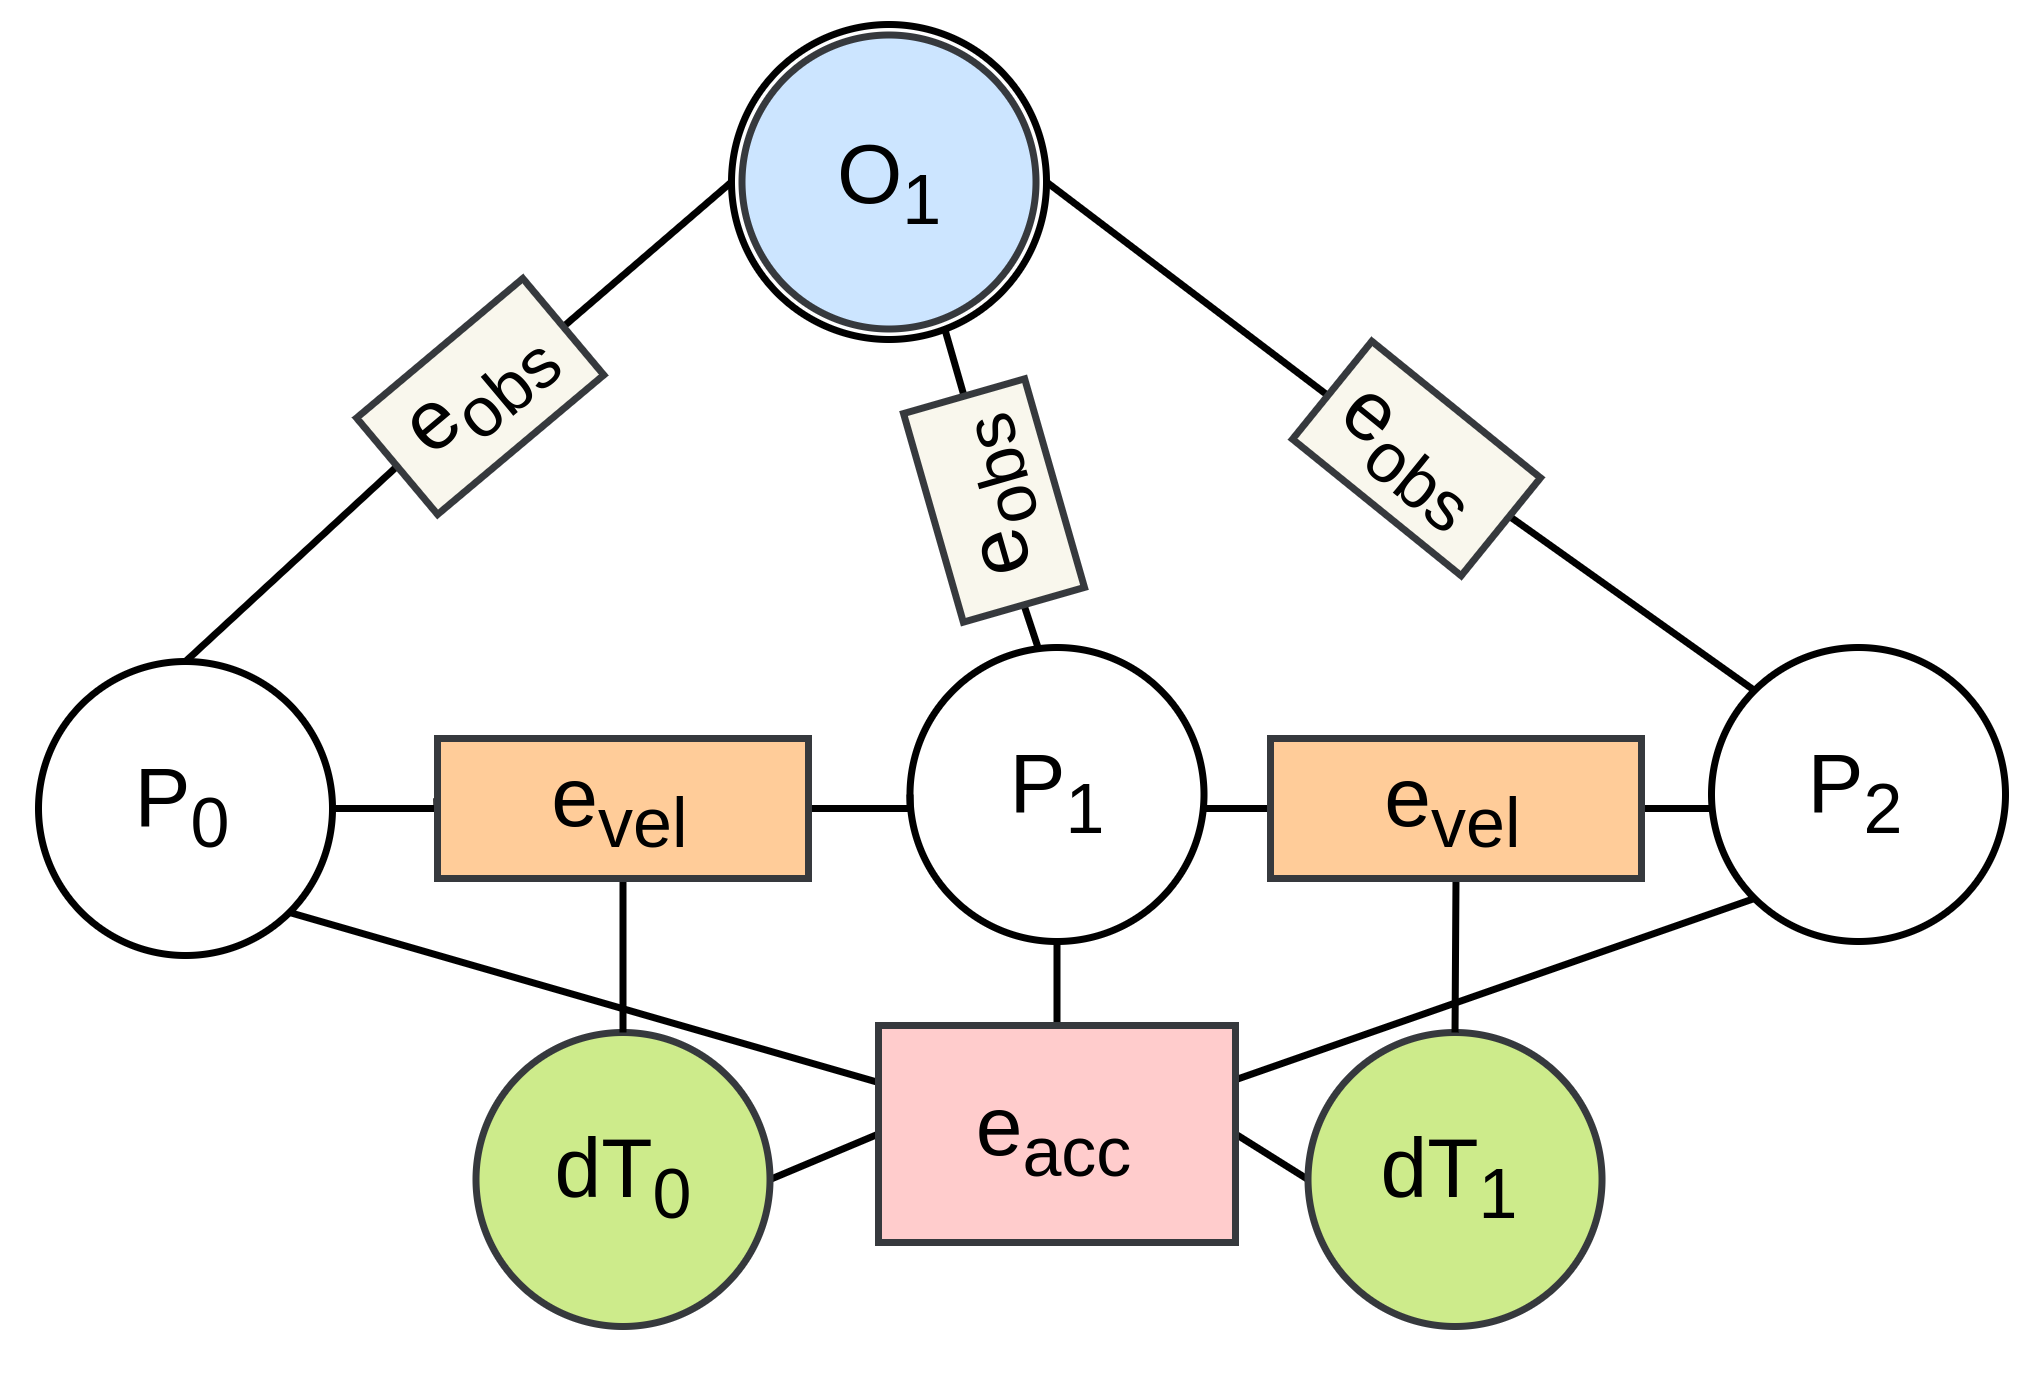
\includegraphics[width=\textwidth]{images/hypergraph_teb.png}
    \caption{Hypergraph used in TEB}
    \end{subfigure}
    \caption{HyperGraph}
    \label{fig:hypergraph}
\end{figure}
Mathematically, if $H$ is a hypergraph and $V$ is the set of vertices and $E$ is the set of hyperedges, then
\begin{equation}
    H = (V, E) \implies E = \{e_i \mid e_i \subseteq V\} \forall i \in I
\end{equation}
where, $I$ is a finite set of indices. An example of a hypergraph is presented in Fig. \ref{fig:hypergraph} (a) with six vertices and four edges. Hypergraphs can contain different kinds of vertices and edges. In Fig. \ref{fig:hypergraph} (a) each edges is of different kind (different colours) and there are two different types of vertices (yellow and white). 

Using hyperedges any mathematical relationship between any of vertices can be defined and this plays an important role in the HAN system proposed in this paper. Therefore hyperedges can naturally be employed to model the kinodynamic constraints of the robot, and so, TEB is modelled using a hypergraph. The vertices of this hypergraph are the poses and the time differences, while the hyperedges represent different constraints or relations between these vertices. A small part of this hypergraph is presented in Fig. \ref{fig:hypergraph} (b), containing five vertices (three poses and two time differences) and shows the velocity, acceleration and obstacle edges. The obstacle is shown in blue with concentric circles. From this figure, it can be seen that the constraints are mostly local as they depend only on a few number of consecutive configurations. This is also the case for majority of the components in the objective function, $f(B)$ of TEB and hence, the TEB hypergraph has a sparse system matrix. Finally, TEB is optimized using the open-source graph optimization framework, g2o. 

\subsubsection{g2o Optimization}
g2o (or General Graph Optimization) \cite{grisetti2011g2o} is an optimization framework developed for solving graph-based nonlinear error function. It offers solutions to the problems with the following structure:
\begin{equation}
\label{eq_optim}
  \mathbf{F(x)} = \sum_{k=\langle i,j \rangle} \mathbf{e}_k(\mathbf{x}_i, \mathbf{x}_j, \mathbf{z}_{ij})^T \mathbf{\Omega}_k\mathbf{e}_k(\mathbf{x}_i, \mathbf{x}_j, \mathbf{z}_{ij}) 
\end{equation}
\begin{equation}
    \mathbf{x}^* = \argmin_\mathbf{x} \mathbf{F(x)}
\end{equation}
where $\mathbf{x}$ represents the parameters to be optimized, $\mathbf{x}_i$, $\mathbf{x}_j$ are the block parameters and $\mathbf{z}_{ij}$ denotes the constraint between them. $\mathbf{\Omega}_k$ denotes the information matrix between the constraints and $\mathbf{e}_k(\mathbf{x}_i, \mathbf{x}_j, \mathbf{z}_{ij})$ is the error vector between the parameters and the constraint. Finally, the optimized set of parameters is represented by $\mathbf{x}^*$. Note that, the part inside the summation in Eq. \eqref{eq_optim} becomes $\Omega_k e_k^2$ if the error is scalar. In case of TEB \cite{rosmann2013efficient}, the objective function, $f(B)$ takes the above form where $B$ is the set of parameters to be optimized, $\mathbf{x}$, $\alpha_k = \Omega_k$, $e_k = \sqrt{f_k}$ and $\mathbf{x}_i = (p_i, \delta t_i)$. g2o uses the Levenberg-Marquardt method to optimize the objective function numerically and offers two Cholesky decomposition solvers, CHOLMOD and CSparse to solve it efficiently.
\subsection{Human-Aware Timed Elastic Bands for Proactive Planning}
In this section, we present the idea of Human-Aware Timed Elastic Band (HATEB), proposed in \cite{khambhaita2017viewing} that lays the basis for this thesis. We briefly discuss how the objective function and hypergraph are modified to include human-aware constraints in robot navigation. 
% \subsubsection{HATEB Formulation: Dual Bands and Proactive Planning}
\subsubsection{HATEB Formulation and Hypergraph}
The idea of HATEB is to add elastic bands to all the humans in the robot's vicinity in addition to the robot and jointly optimize the robot and the human trajectories in terms of kinodynamic and human-aware (or social) constraints. This gives rise to a multivariate multi-objective optimization problem to solve and the same weighted sum approach proposed in TEB is used for HATEB as well. Therefore, if the robot's band is represented by $B_r$ and the human bands by $\{B_{h_k}\}_{k=0}^n$ when $n (\in \mathbb{N})$ humans are present in the vicinity, the new objective function to solve is,
\begin{equation}
    \label{hateb_eq}
    f(B_r, B_{h_0}...B_{h_n}) = \underbrace{\sum_{i}\alpha_i f_i(B_r)}_{F_R} + \sum_k \left (\underbrace{\sum_{j}\alpha_j f_j(B_{h_k})}_{F_H} + \underbrace{\sum_l \alpha_l f_l(B_r, B_{h_k})}_{F_S} \right )
\end{equation}
\begin{equation}
    B_r^*, B_{h_0}^*...B_{h_n}^* = \argmin_{B_r, B_{h_0}...B_{h_n}} f(B_r, B_{h_0}...B_{h_n})
\end{equation}
where $B_r^*, \{B_{h_k}^*\}_{k=0}^n$ are optimized trajectories for the robot and the humans respectively. The initial paths of humans for this optimization is obtained from the human path prediction module of the system.
\begin{figure}[!h]
    \centering
    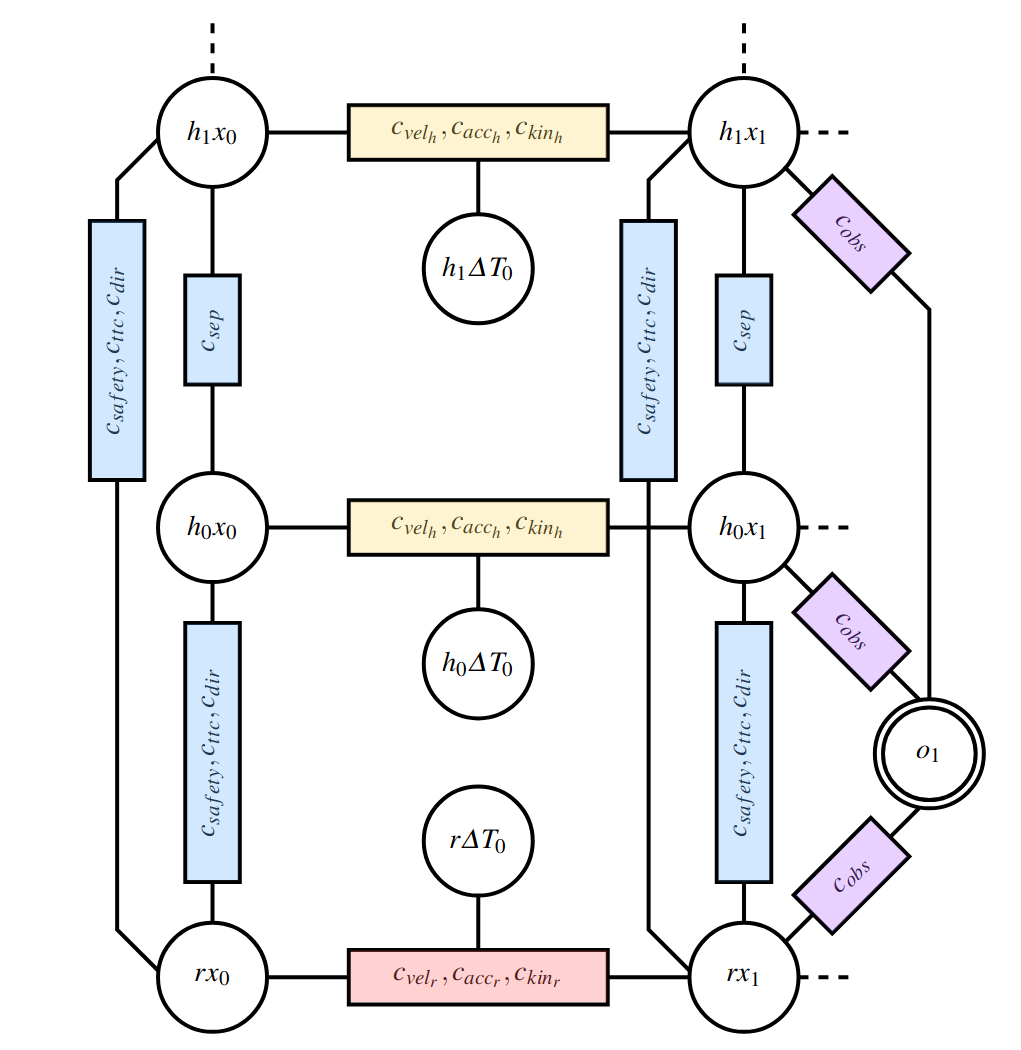
\includegraphics[width=0.65\columnwidth]{images/hateb_new.png}
    \caption{The updated hypergraph of HATEB~\cite{khambhaita2017viewing}. There are 3 bands, one for the robot and the other two for humans. The kinodynamic constraints are shown as horizontal edges (yellow, red), social constraints are shown as vertical edges (blue) and the obstacle avoidance constraints are shown as diagonal edges (purple).}
    \label{fig:hateb_hypergraph}
\end{figure}

In Eq.~\ref{hateb_eq}, $F_R$ and $F_H$ represent the objective functions for the robot and human trajectories whereas, $F_S$ denotes the objective for human-robot social constraints. All these constraints are represented as hyperedges of an updated hypergraph and a small part of this hypergraph is shown in Fig. \ref{fig:hateb_hypergraph}. The social constraints between human-robot and human-human are highlighted in blue while the kinodynamic constraints of the robot and humans are highlighted in red and yellow respectively. Finally, the obstacles constraints are shown in purple. Even though the system matrix is still sparse, it is denser than before and as we keep adding bands for humans, the density grows and the trajectories cannot be obtained in real-time. 

\newpage
\subsubsection{Proactive Planning and Social constraints}
The joint optimization produces the robot trajectory that obeys the social norms implemented in $F_S$. Further, the combined human-robot trajectories planning makes the robot proactively estimate humans' plans and quickly adapt its trajectory before it is too late. This idea of adding double-sided (robot side, human side) bands is called `{\textit{Dual Band}}' throughout this thesis. This approach always elicits solutions, if they exist, for all agents which can solve any navigation situation if every agent follows the solution. 
Using the above architecture, three social constraints are defined, 1) \textit{Human-Robot Safety}, which takes care of human safety and proxemics, 2) \textit{Time-to-Collision (TTC)}, which adds early intention show to the robot's trajectory and 3) \textit{Directional}, that tries to establish a trade-off between slowing down and changing the path. In HATEB, the objective function for safety clearance from obstacles is also updated to make the robot move towards obstacle rather than human in constrained scenarios. All these constraints are added to the objective function as piecewise continuous and differential error functions like in TEB. We believe that this architecture is better suited to HAN than the reactive approaches, especially in intricate indoor scenarios.



\section{Our Approach and Contributions}
One of the noted limitation with \textit{Dual Band} approach is that it assumes that the humans are always co-operative agents and will not cause any deadlock situations. So it always proposes solutions with the assumption that the human will be moving, which might not be the case. When the human stops moving or behaves in an unconventional way, the robot gets stuck without moving or oscillates without making any progress towards the goal. Therefore, we introduce situation assessment over proactive planning as shown in Fig. \ref{fig:full_contrib}. This situation analysis is local and happens at the trajectory planning level. 
\begin{figure}[h!]
    \centering
    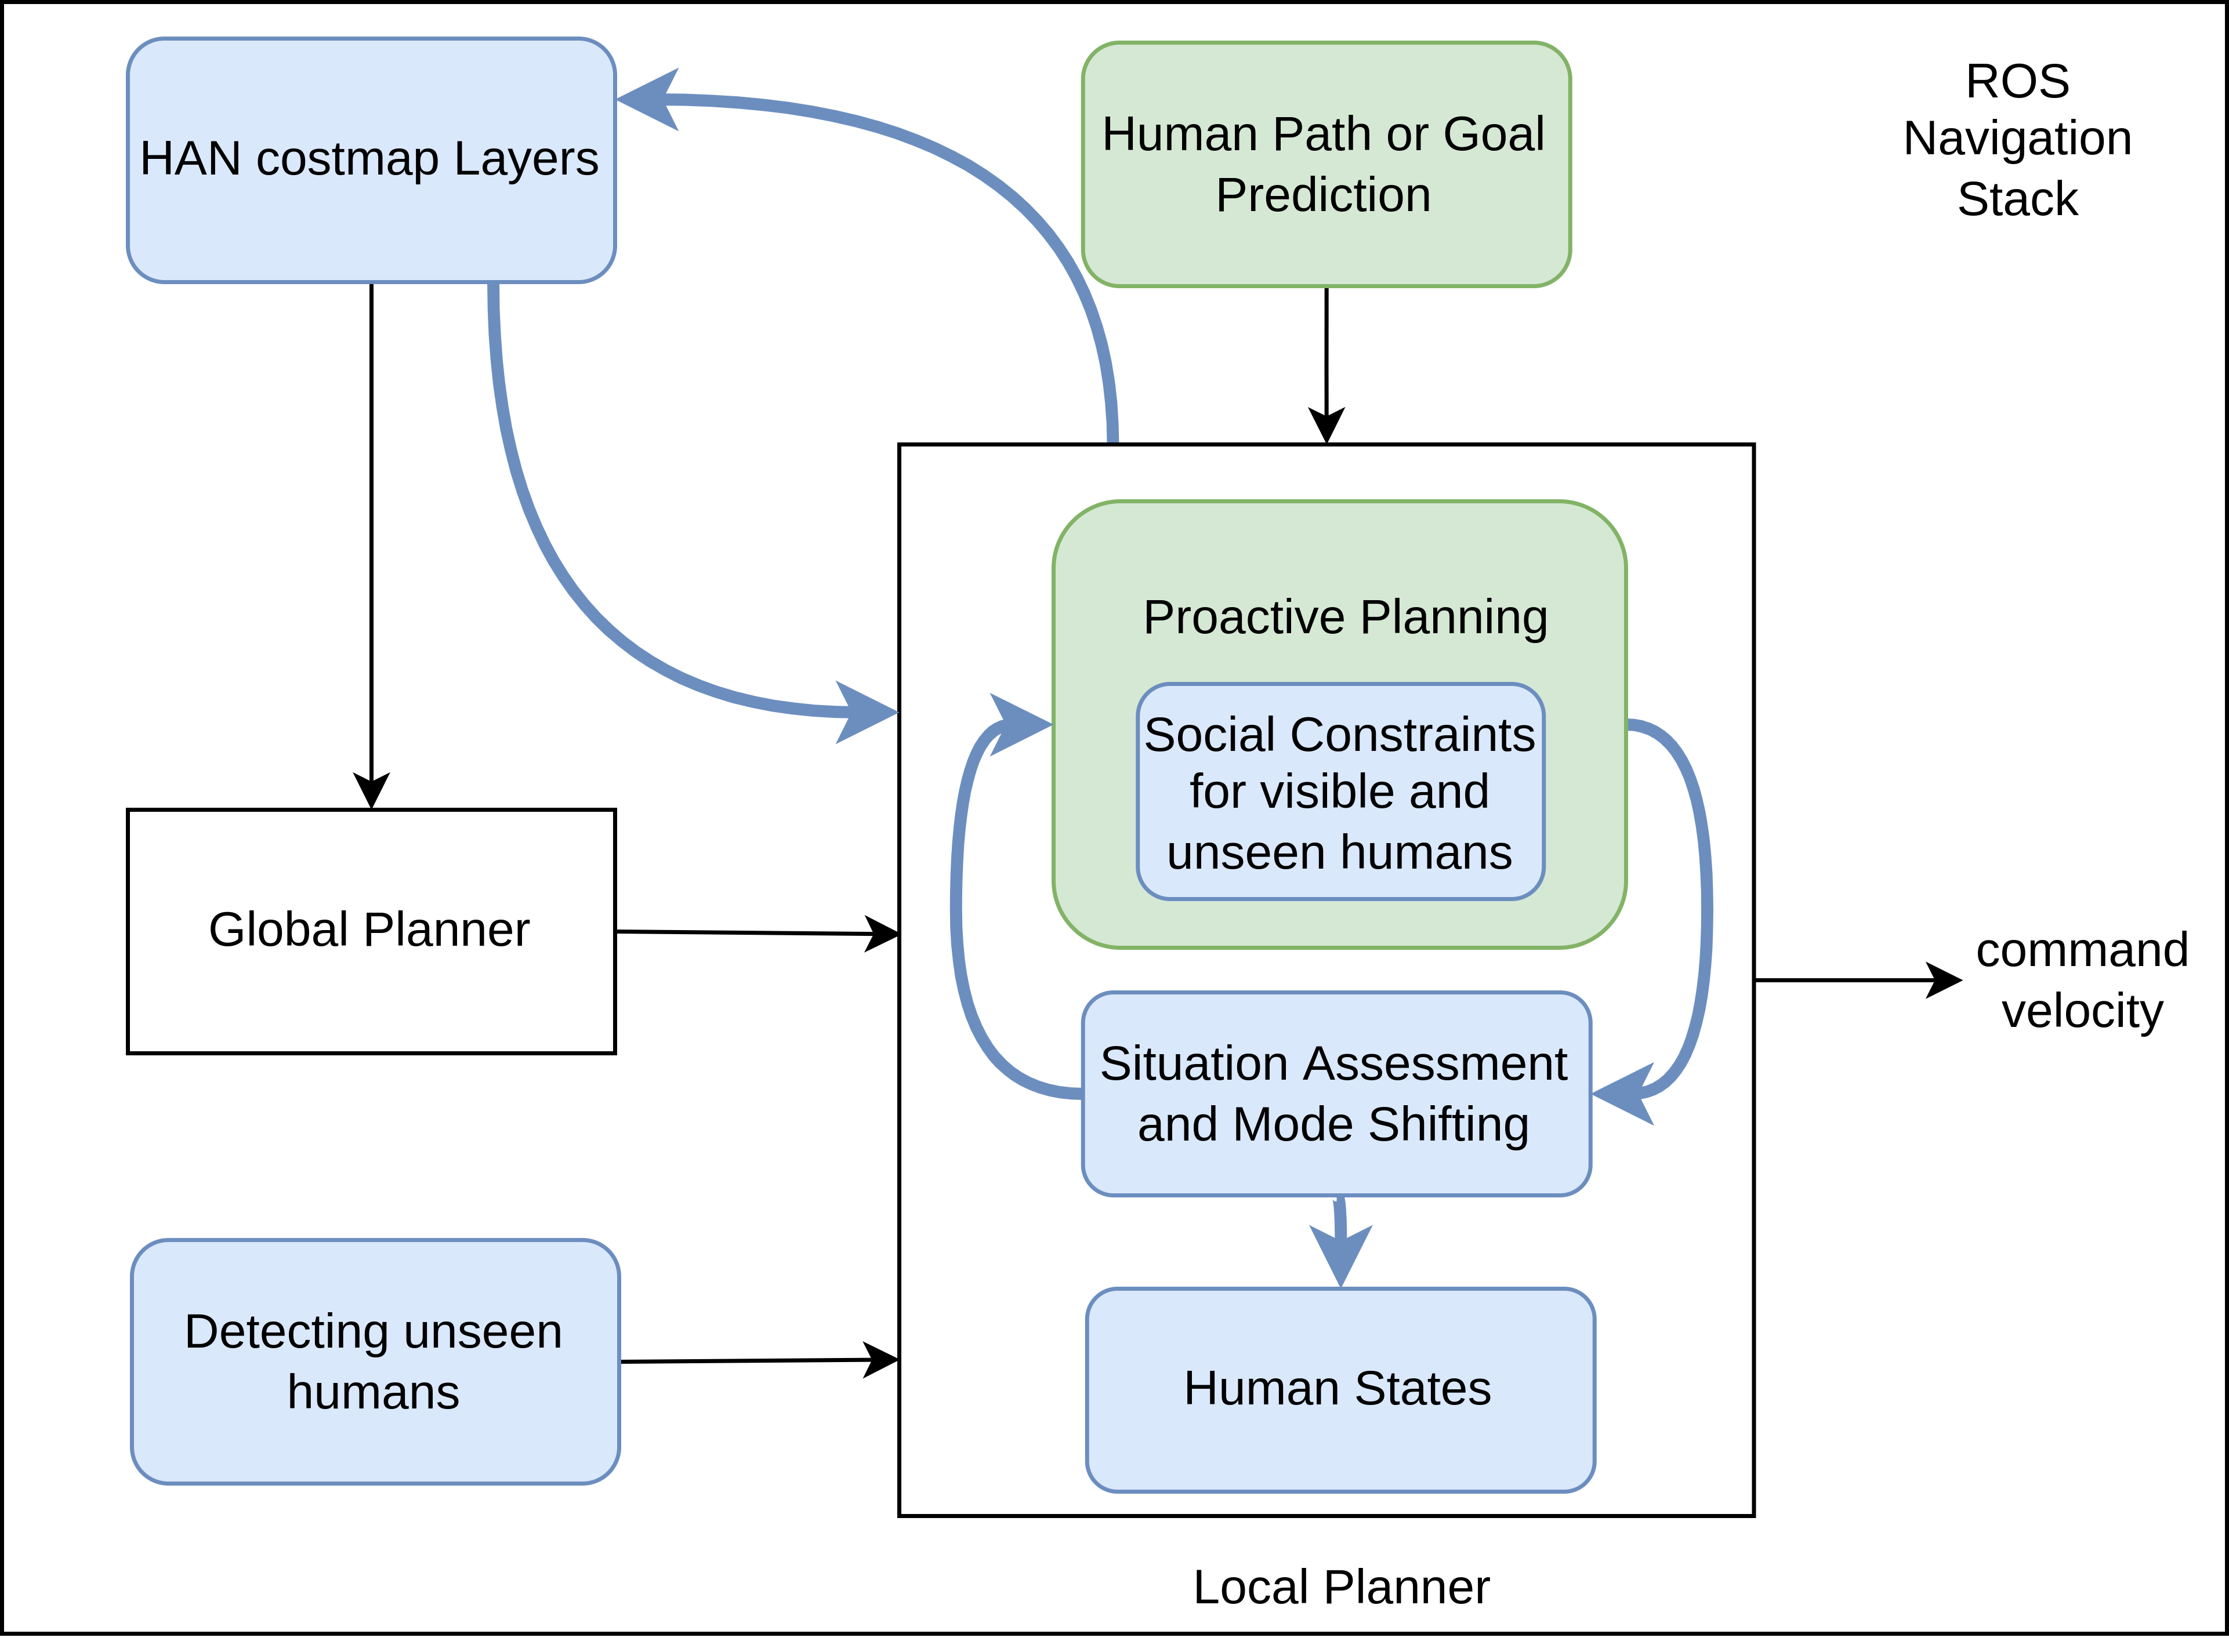
\includegraphics[width=0.8\columnwidth]{images/contrib_new.png}    \caption{The situation assessment module is combined with proactive planning inside the local planner. The system can use any existing global planner.}
    \label{fig:full_contrib}
\end{figure}
After analysing a situation and determining if it's a deadlock or any other uncomfortable setting, we have to find a way to mitigate it. In this thesis, we do this by shifting between different navigation modalities. The blue arrows in the Fig. \ref{fig:full_contrib} represent how the proactive planning, situation assessment and mode shifting are interlinked with each other. The integration of situation analysis into trajectory planning and how mode shifting happens are presented in detail in the subsequent chapters.

The crux of this thesis is finding and mitigating the uncomfortable human-robot interactions in HAN. Note that this includes the humans in view and the humans the robot has not seen yet. The main contributions of this thesis in developing a human-aware ROS navigation stack are shown in coloured boxes in Fig. \ref{fig:full_contrib}. The ones in blue colour represent the novel contributions while the ones in green represent significant modifications over the previous work. The blue arrows stand for the new connections we have made in our proposed HAN. The proactive planning has been significantly improved by proposing new human-robot social constraints for both visible and unseen humans. The updated path prediction module with new goal prediction methodologies further improve the proactive planning and hence better navigation behaviours can be obtained. The new HAN costmap layers are proposed to mainly address the global planning around static humans. However, these layers are designed to update based on the states of humans (blue arrows) given by the local planner and also play a role in trajectory planning. While analysing a situation, the state of the human (static, moving, stopped etc.) is necessary and hence situation assessment modules maintains a list of states for the humans it has encountered during its navigation. The choice of the modality is based on the state of the human as well as the situation. The idea of mitigating collisions with unseen humans is quite new in case of HAN and makes the robot ready to face any kind of situations when combined with our multi-context HAN system proposed in this thesis. We believe that the idea of mode shifting within local planning is significantly new and can be seen as a major contribution as well.

